% \documentclass[a4paper,12pt]{article}

% % Paquetes básicos
% \usepackage[utf8]{inputenc}
% \usepackage[T1]{fontenc}
% \usepackage[spanish]{babel}
% \usepackage{graphicx}
% \usepackage{xcolor}
% \usepackage{lipsum}
% \usepackage{geometry}
% \geometry{top=3cm, bottom=3cm, left=2.5cm, right=2.5cm}

% % Paquetes para diseño
% \usepackage{titlesec}
% \usepackage{fancyhdr}
% \usepackage{amsmath}
% \usepackage{amssymb}
% \usepackage{hyperref}

% % Paquetes para el entorno lstlisting
% \usepackage{listings}
% \usepackage{inconsolata}

% % Paquete para fondo
% \usepackage{background}

% % Configuración de lstlisting
% \lstset{
%     language=Python,
%     basicstyle=\ttfamily\small,
%     keywordstyle=\color{blue}\bfseries,
%     stringstyle=\color{teal},
%     commentstyle=\color{gray}\itshape,
%     numbers=left,
%     numberstyle=\tiny\color{gray},
%     backgroundcolor=\color{black!5},
%     frame=single,
%     rulecolor=\color{black!50},
%     breaklines=true,
%     captionpos=b,
%     showstringspaces=false
% }

% % Configuración de título
% \titleformat{\section}{\normalfont\Large\bfseries}{\thesection}{1em}{}
% \usepackage{mathpazo}

% %encabezado y pie de página nivel profesional
% \usepackage{fancyhdr}
% \pagestyle{fancy}
% \fancyhf{}
% \fancyhead[L]{\leftmark}
% \fancyhead[R]{\rightmark}
% \fancyfoot[C]{\thepage}
% \fancyfoot[R]{\textbf{       (UGR)} \today}



% % Información del documento
% \title{
%     \vspace{-2cm}
%     
\includegraphics[width=0.3\textwidth]{images/fccee.jpg} \\ % Cambia el logo si es necesario
%     \LARGE Ingeniería Informática + ADE\\
%     \large Universidad de Granada (UGR)\\[1cm]
% }
% \author{\textbf{Autor:} Ismael Sallami Moreno}
% \date{\textbf{Asignatura:} Resolución de los Ejercicios Propuestos Reueltos Tema 5: Inmovilizaciones materiales}

% % Configuración del fondo
% \backgroundsetup{
%     scale=1,
%     color=black,
%     opacity=0.2,
%     angle=0,
%     position=current page.south,
%     vshift=0pt,
%     hshift=0pt,
%     contents={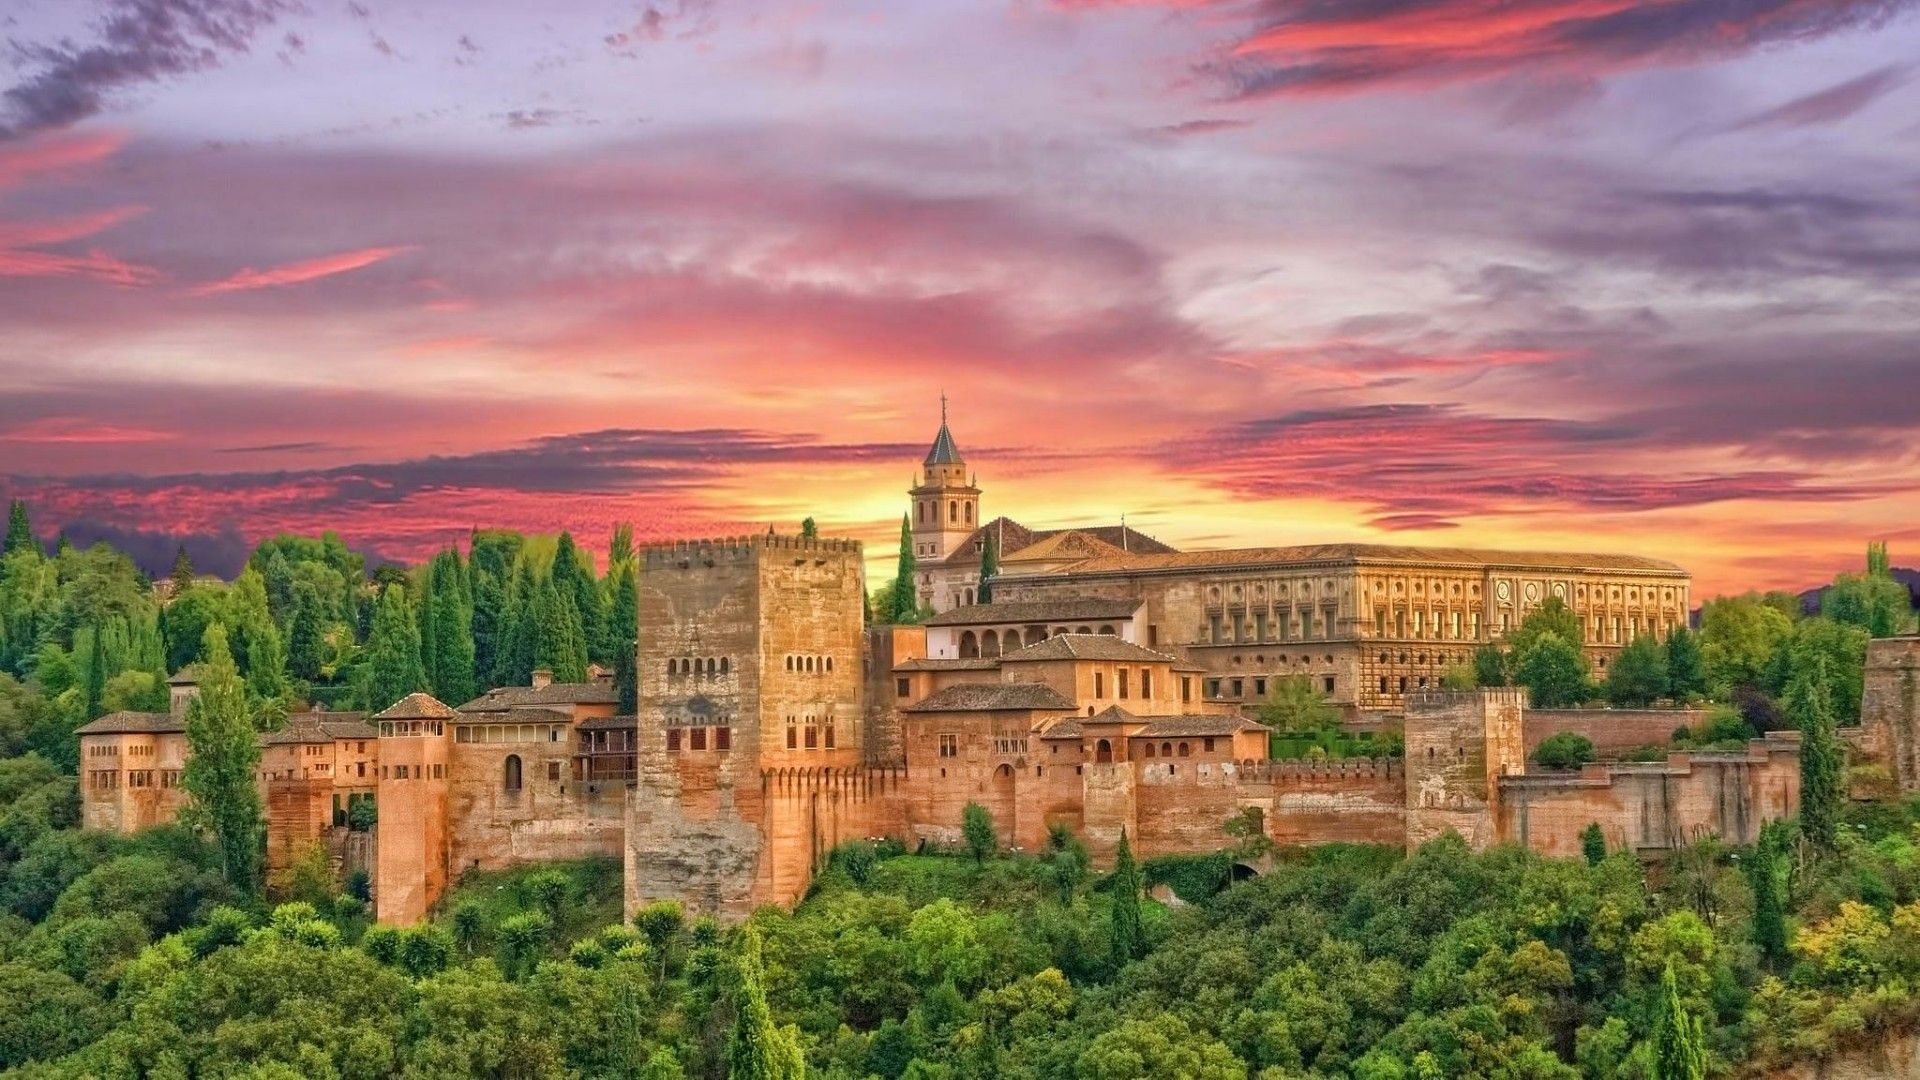
\includegraphics[width=\paperwidth,height=\paperheight,keepaspectratio]{images/granada.jpg}}
% }


\documentclass[a4paper,12pt]{article}

% Paquetes básicos
\usepackage[utf8]{inputenc}
\usepackage[T1]{fontenc}
\usepackage[spanish]{babel}
\usepackage{graphicx}
\usepackage{xcolor}
\usepackage{lipsum}
\usepackage{geometry}
\geometry{top=3cm, bottom=3cm, left=2.5cm, right=2.5cm}

% Paquetes para diseño
\usepackage{titlesec}
\usepackage{fancyhdr}
\usepackage{amsmath}
\usepackage{amssymb}
\usepackage{hyperref}
\usepackage{tcolorbox}
\usepackage{float}

% Paquetes para el entorno lstlisting
\usepackage{listings}
\usepackage{inconsolata}

\usepackage{tocbibind} % Para incluir subsubsubsections en el índice
\usepackage{titlesec}  % Para ajustar la numeración de las secciones
\setcounter{tocdepth}{5} % Ajusta la profundidad del índice
\setcounter{secnumdepth}{5} % Ajusta la profundidad de la numeración

% Configuración de la numeración para \paragraph
\titleformat{\paragraph}
{\normalfont\normalsize\bfseries}{\theparagraph}{1em}{}
\titlespacing*{\paragraph}{0pt}{3.25ex plus 1ex minus .2ex}{1.5ex plus .2ex}

% Paquete para fondo
\usepackage{background}

\newcommand{\fec}{31/12/}
\newcommand{\AIM}{681 Amortización del inmovilizado material }
\newcommand{\AAMAQ}{2813 Amortización acumulada de maquinaria }
\newcommand{\valorrecuperable}{Valor recuperable = max\{valor neto realizable, valor en uso\} =}
\newcommand{\PDI}{691 Pérdidas por deterioro de inmovilizado material}
\newcommand{\DVM}{2913 Deterioro del valor de la maquinaria }
\newcommand{\RDIM}{791 Reversión deterioro inmovilizado material}
\newcommand{\VC}{Valor contable = }
\newcommand{\PPIM}{671 Pérdidas procedentes del inmovilizado material}
\newcommand{\bancos}{572 Bancos cuenta corriente}
\newcommand{\cuotaamort}{Cuota de amortización = }
\newcommand{\enajenacion}{543 Créditos a corto plazo por enajenación del inmovilizado}
\newcommand{\benefIM}{771 Beneficios procedentes del inmovilizado material}
\usepackage{amsmath}
\newcommand{\myequation}[2]{\ensuremath{\frac{#1}{#2}}}
\newcommand{\flechita}{$\rightarrow$}
\newcommand{\deterioropatente}{2903 Deterioro de valor de la propiedad industrial}
\newcommand{\perdidasdelintangible}{690 Pérdidas por inmovilizado intangible}
\newcommand{\amortAcumPatente}{2803 Amortización acumulada de la propiedad industrial}
\newcommand{\trabajosrealizadosII}{730 Trabajos realizados para el inmovilizado intangible}
\newcommand{\cursiva}[1]{\textit{#1}}
\newcommand{\negrita}[1]{\textbf{#1}}
%comandos extra
\newcommand{\cuenta}[1]{
    \ifnum#1=2800 2800. Amortización acumulada de investigación\fi
    \ifnum#1=2801 2801. Amortización acumulada de desarrollo\fi
    \ifnum#1=2802 2802. Amortización acumulada de concesiones administrativas\fi
    \ifnum#1=2803 2803. Amortización acumulada de propiedad industrial\fi
    \ifnum#1=2804 2804. Amortización acumulada de fondo de comercio\fi
    \ifnum#1=2805 2805. Amortización acumulada de derechos de traspaso\fi
    \ifnum#1=2806 2806. Amortización acumulada de aplicaciones informáticas\fi
    \ifnum#1=2811 2811. Amortización acumulada de construcciones\fi
    \ifnum#1=2812 2812. Amortización acumulada de instalaciones técnicas\fi
    \ifnum#1=2813 2813. Amortización acumulada de maquinaria\fi
    \ifnum#1=2814 2814. Amortización acumulada de utillaje\fi
    \ifnum#1=2815 2815. Amortización acumulada de otras instalaciones\fi
    \ifnum#1=2816 2816. Amortización acumulada de mobiliario\fi
    \ifnum#1=2817 2817. Amortización acumulada de equipos para procesos de información\fi
    \ifnum#1=2818 2818. Amortización acumulada de elementos de transporte\fi
    \ifnum#1=2819 2819. Amortización acumulada de otro inmovilizado material\fi
    \ifnum#1=282 282. Amortización acumulada de las inversiones inmobiliarias\fi
    \ifnum#1=280 280. Amortización acumulada del inmovilizado intagible\fi
    \ifnum#1=281 281. Amortización acumulada del inmovilizado material\fi
}


% Configuración de lstlisting
\lstset{
    language=Python,
    basicstyle=\ttfamily\small,
    keywordstyle=\color{blue}\bfseries,
    stringstyle=\color{teal},
    commentstyle=\color{gray}\itshape,
    numbers=left,
    numberstyle=\tiny\color{gray},
    backgroundcolor=\color{black!5},
    frame=single,
    rulecolor=\color{black!50},
    breaklines=true,
    captionpos=b,
    showstringspaces=false
}

% Configuración de título
\titleformat{\section}{\normalfont\Large\bfseries}{\thesection}{1em}{}

% Información del documento
\title{
    \vspace{-2cm}
    
\includegraphics[width=0.3\textwidth]{images/fccee.jpg} \\ % Cambia el logo si es necesario
    \LARGE Ingeniería Informática + ADE\\
    \large Universidad de Granada (UGR)\\[1cm]
}
\author{\textbf{Autor:} Ismael Sallami Moreno}
\date{\textbf{Asignatura:} Resolución de los Ejercicios Propuestos Reueltos Tema 6: Inmovilizado Intangible
}
\usepackage{mathpazo}
\usepackage{fancyhdr}
\pagestyle{fancy}
\fancyhf{}
\fancyhead[L]{\leftmark}
\fancyhead[R]{\rightmark}
\fancyfoot[C]{\thepage}
\fancyfoot[R]{\textbf{       (UGR)} \today}
\usepackage{enumitem}

\usepackage{tcolorbox}

% Configuración del fondo
\backgroundsetup{
    scale=1,
    color=black,
    opacity=0.2,
    angle=0,
    position=current page.south,
    vshift=0pt,
    hshift=0pt,
    contents={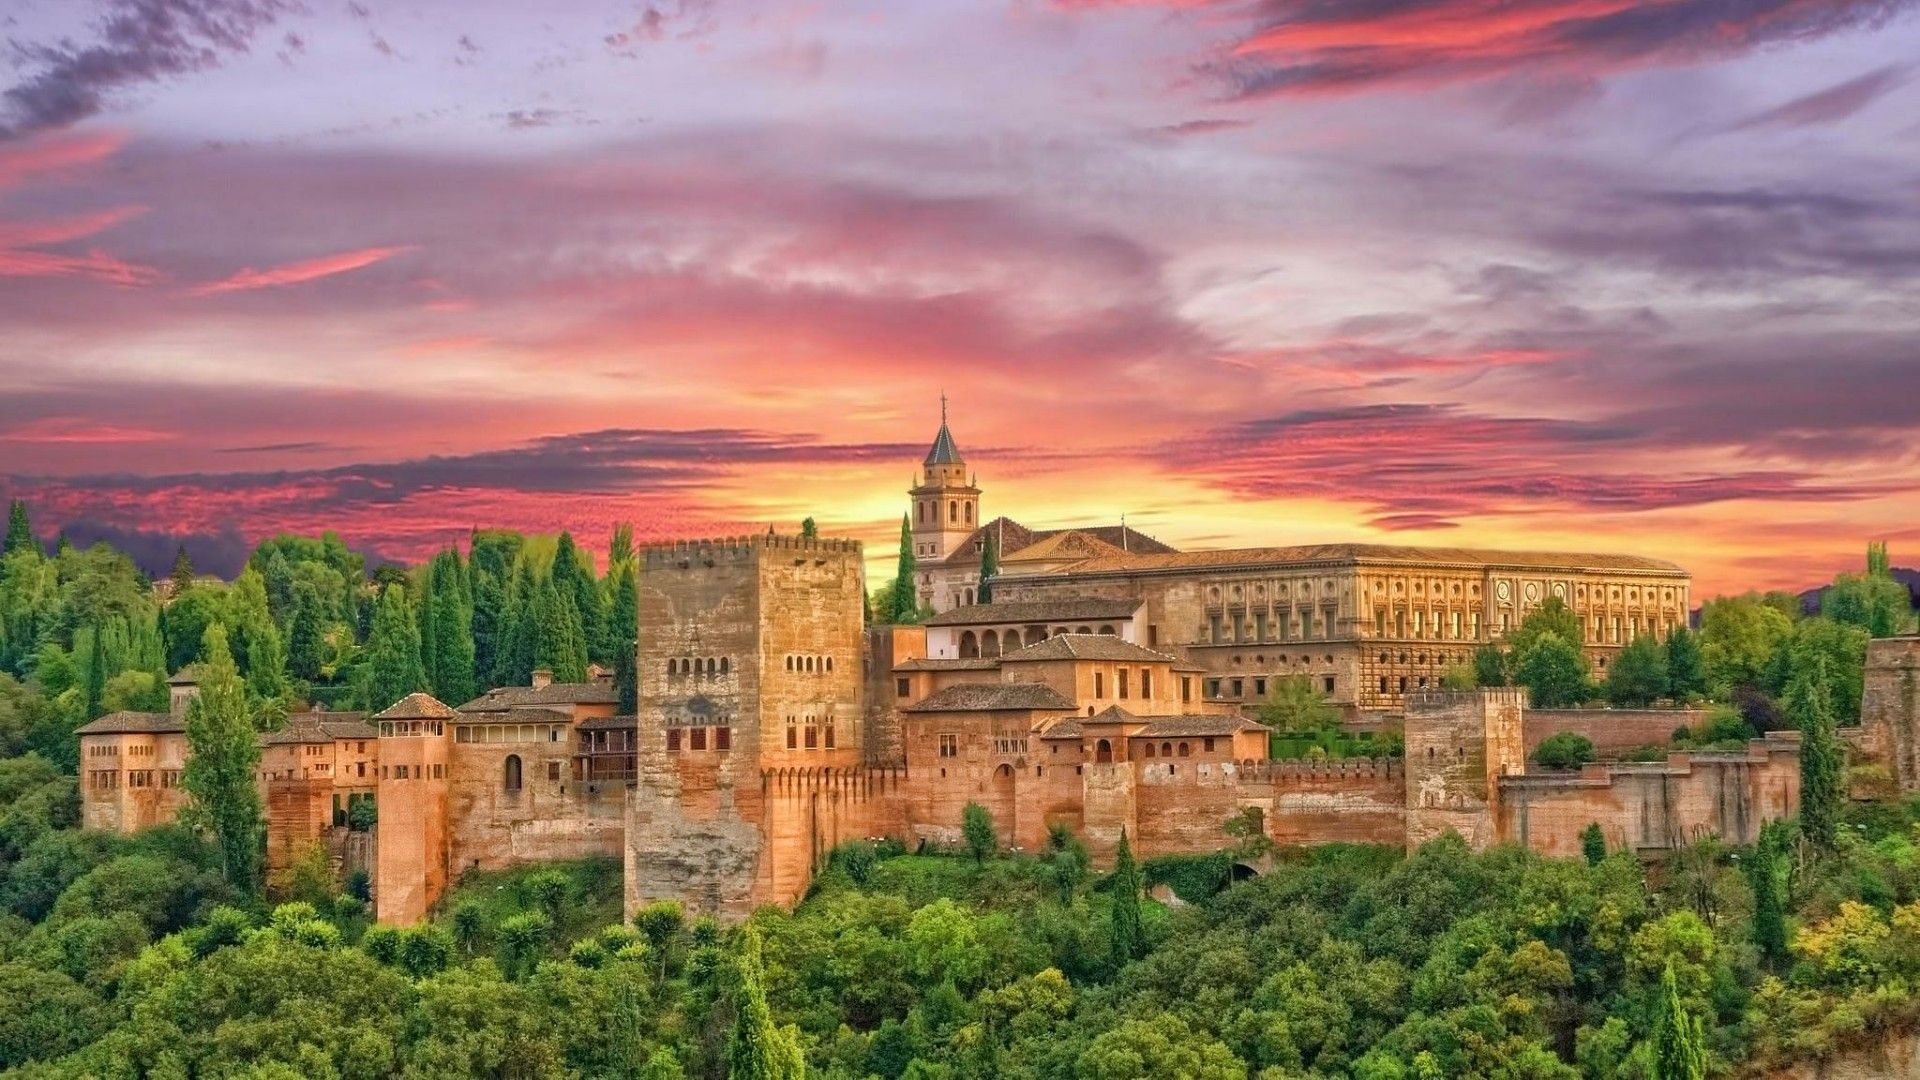
\includegraphics[width=\paperwidth,height=\paperheight,keepaspectratio]{images/granada.jpg}}
}

% Inicio del documento
\begin{document}

% Portada
\maketitle
\thispagestyle{empty}

\begin{center}
    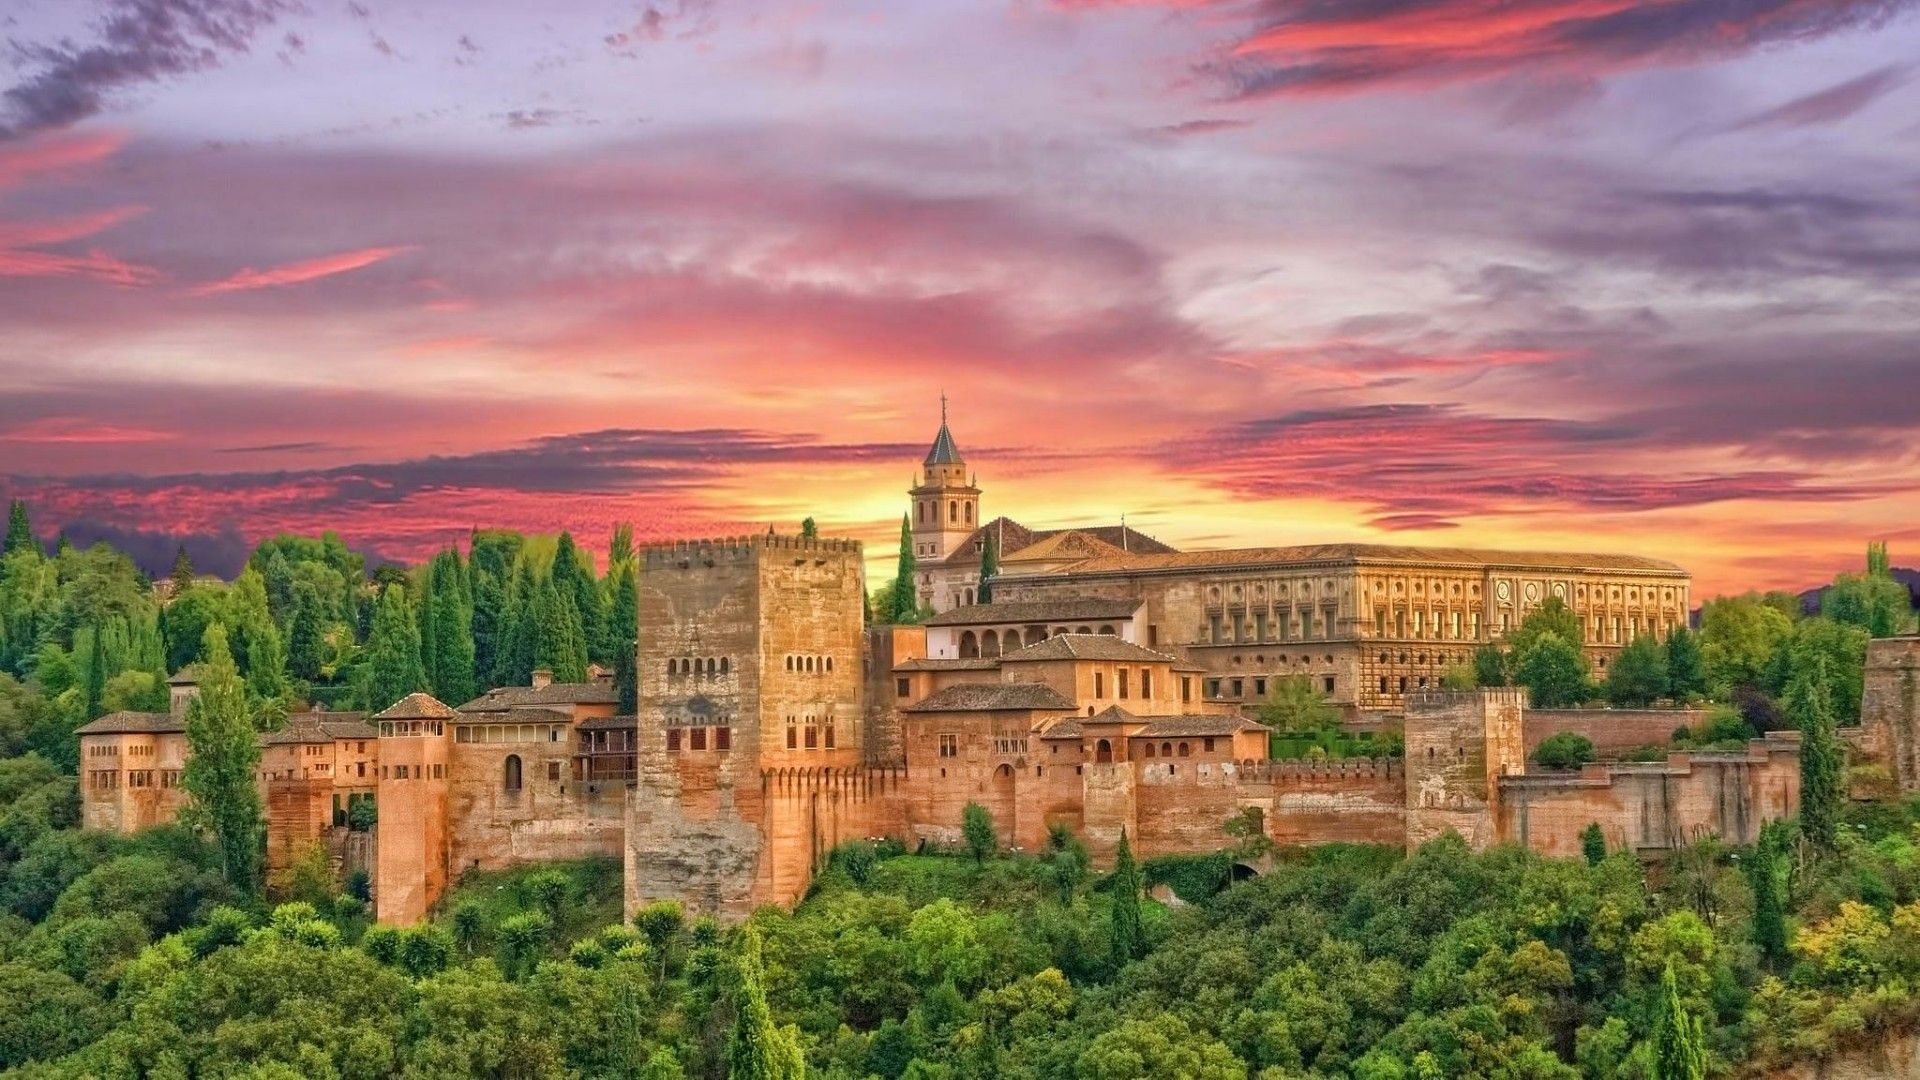
\includegraphics[width=\textwidth,height=0.4\textheight,keepaspectratio]{images/granada.jpg} \\ % Añade tu imagen de fondo
    \vfill
\end{center}

\newpage

% Índice (opcional)
\tableofcontents
\newpage

\section{Ejercicio 1}

\begin{table}[H]
    \centering
    \begin{tabular}{|p{3cm}|p{6cm}|p{3cm}|}
    \hline
    \textbf{DEBE} & \textbf{operaciones de la compra de la patente a 1/10/2017} & \textbf{HABER} \\
    \hline
    200.000 & 203  Propiedad industrial & \\
    \hline
    & \bancos & 200.000\\
    \hline
    \end{tabular}
\end{table}

\begin{itemize}
    \item \valorrecuperable \{114.00, 110.000\} = 114.000
    \item \textbf{La vida útil de la patente se acorta a 3 años a partir de este momento}
    \item \cuotaamort \myequation{200000}{8} = 25.000
    \item \VC 200.000 - 25.000·\myequation{3}{12}(2017) - 25.000 (2018) - 25.000 (2019) - 25.000 (2020) = 118.750
    \item Deterior de la patente = 118.750 - 114.000 = 4.750
\end{itemize}

\begin{table}[H]
    \centering
    \begin{tabular}{|p{3cm}|p{6cm}|p{3cm}|}
    \hline
    \textbf{DEBE} & \textbf{correción valorativa de carácter reversible el 31/12/2020} & \textbf{HABER} \\
    \hline
    4750& 690 Pérdidas por inmovilizado intangible& \\
    \hline
    & 2903 Deterioro de valor de la propiedad industrial&4750 \\
    \hline
    \end{tabular}
\end{table}

\begin{itemize}
    \item Al haber deterioro debemos de recalcular el valor de la amortización.
    %\item Los meses que quedan son: 96 (8 años) - los tres años amortizados 3*12 - 3 meses de 2017 = 57 meses 
    % \item \cuotaamort 118.750 - 4750 = \myequation{114000}{57 \text{ meses}} = 2000 cada mes 
    %\item De 2021 han pasado 6 meses, por lo que la amortización de 2021 es 2000·6 = 12.000
    \item \cuotaamort \myequation{114000}{3} = 38.000 cada año
    \item De 2021 han pasado 6 meses, por lo que la amortización de 2021 es 38.000/2 = 19.000
    \item La Amortización total de la patente es = 200.000 - 118.750 = 81.250 + (la de 2021) = 81.250 + 19.000 = 100.250 
\end{itemize}

\begin{table}[H]
    \centering
    \begin{tabular}{|p{3cm}|p{6cm}|p{3cm}|}
    \hline
    \textbf{DEBE} & \textbf{venta de la patente el 1/7/2021} & \textbf{HABER} \\
    \hline
    100.250 & 2803 Amortización acumulada de la propiedad industrial& \\
    \hline
    4.750 & 2903 Deterioro de valor de la propiedad industrial& \\
    \hline
    100.000& \bancos & \\
    \hline
    & 203 Propiedad Industrial& 200.000\\
    \hline
    & \textbf{770 Beneficios procedentes del Inmovilizado Intangible}& 5.000\\
    \hline
    \end{tabular}
\end{table}

\section{Ejercicio 2}

\begin{table}[H]
    \centering
    \begin{tabular}{|p{3cm}|p{6cm}|p{3cm}|}
    \hline
    \textbf{DEBE} & \textbf{a \fec2016 activación de gastos imputables al Proyecto A} & \textbf{HABER} \\
    \hline
    10.000 & 620 gastos de investigación y desarrollo del ejercicio& \\
    \hline
    & \bancos & 10.000\\
    \hline
    10.000& 200 Investigación& \\
    \hline
    & 730 Trabajos realizados para el inmovilizado intangible&  10.000\\
    \hline
    \end{tabular}
\end{table}



\begin{table}[H]
    \centering
    \begin{tabular}{|p{3cm}|p{6cm}|p{3cm}|}
    \hline
    \textbf{DEBE} & \textbf{a \fec2017 activación de los gastos imputables al Proyecto B} & \textbf{HABER} \\
    \hline
    2.500 & 620 gastos de investigación y desarrollo del ejercicio& \\
    \hline
    & \bancos & 2.500\\
    \hline
    2.500& 200 Investigación& \\
    \hline
    & 730 Trabajos realizados para el inmovilizado intangible&  2.500\\
    \hline
    \end{tabular}
\end{table}

\begin{itemize}
    \item \cuotaamort \myequation{2500}{5 \text{ años}} = 500
\end{itemize}

\begin{table}[H]
    \centering
    \begin{tabular}{|p{3cm}|p{6cm}|p{3cm}|}
    \hline
    \textbf{DEBE} & \textbf{a \fec2019 Amortización EXCLUSIVAMENTE de los gastos del desarrollo del Proyecto A} & \textbf{HABER} \\
    \hline
    500 & 680 Amortización del Inmovilizado Intangible& \\
    \hline
    & 2801 Amortización Acumulada de \textit{desarrollo}& 500\\
    \hline
    \end{tabular}
\end{table}

\begin{itemize}
    \item \cuotaamort \myequation{2500}{5 \text{ años}} = 500
\end{itemize}

\begin{table}[H]
    \centering
    \begin{tabular}{|p{3cm}|p{6cm}|p{3cm}|}
    \hline
    \textbf{DEBE} & \textbf{\fec2019 amortización de los gastos activados del Proyecto B} & \textbf{HABER} \\
    \hline
    500 & 680 Amortización del Inmovilizado Intangible& \\
    \hline
    & 2800 Amortización Acumulada de \textit{Investigación}& 500\\
    \hline
    \end{tabular}
\end{table}

\begin{table}[H]
    \centering
    \begin{tabular}{|p{3cm}|p{6cm}|p{3cm}|}
    \hline
    \textbf{DEBE} & \textbf{\fec2020 activación de los gastos imputables del Proyecto A} & \textbf{HABER} \\
    \hline
    3.000 & 620 gastos de investigación y desarrollo del ejercicio& \\
    \hline
    & \bancos & 3.000\\
    \hline
    3.000& 200 Investigación& \\
    \hline
    & 730 Trabajos realizados para el inmovilizado intangible&  3.000\\
    \hline
    \end{tabular}
\end{table}

\begin{table}[H]
    \centering
    \begin{tabular}{|p{3cm}|p{6cm}|p{3cm}|}
    \hline
    \textbf{DEBE} & \textbf{\fec2020 inscripción de la patente resultante del Proyecto A} & \textbf{HABER} \\
    \hline
    Lo restante = 7.500& 203 Propiedad Industrial& \\
    \hline
    $500 (2018)+1000(2019)$& 2801 Amortización acumulada de desarrollo& \\
    \hline
    & \bancos & 1.000\\
    \hline
    & 201 desarrollo& 8.000 = 5.000 (2.500 de 2018 y 2019) + 3.000 de 2020\\
    \hline
    \end{tabular}
\end{table}

\begin{table}[H]
    \centering
    \begin{tabular}{|p{3cm}|p{6cm}|p{3cm}|}
    \hline
    \textbf{DEBE} & \textbf{\fec2020 Finalización sin exito del Proyecto B} & \textbf{HABER} \\
    \hline
    & 200 Investigación& 10.000 = 2.500 por 4 años, desde 2016 hasta 2020\\
    \hline
    5.000 = 500 + 1.000 + 1.500 + 2.000 (de 4 años)& 2800 Amortización Acumulada de de Investigación& \\
    \hline
    5.000 = lo restante& \perdidasdelintangible& \\
    \hline
    \end{tabular}
\end{table}

\section{Ejercicio 3}

\begin{table}[H]
    \centering
    \begin{tabular}{|p{3cm}|p{6cm}|p{3cm}|}
    \hline
    \textbf{DEBE} & \textbf{Reconocimiento contable inicial de al adquisición de la UGE} & \textbf{HABER} \\
    \hline
    900.000& 213 maquinaria& \\
    \hline
    300.000& 216 mobiliario& \\
    \hline
    & 400 Proveedores & 200.000\\
    \hline
    & \bancos & 1.100.000\\
    \hline
    100.000& 204 Fondo de Comercio& \\
    \hline
    \end{tabular}
\end{table}

\begin{itemize}
    \item \valorrecuperable 1.000.000
    \item Valor contable de la UGE:
    \begin{itemize}
        \item Fondo de comercio = \cuotaamort \myequation{100.000}{10} = 10.000 \flechita \VC 100.000 - 10.000 = 90.000
        \item Proveedores \flechita nada porque se supone que ya se pagó en Febrero.
    \end{itemize}
    \item TOTAL = 810.000 + 270.000 + 90.000 = 1.170.000
    \item Deterioro = 1.170.000 - 1.000.000 = 170.000
    \item No hay suficiente fondo de comercio para cubrir el deterioro, por lo que se reparte entre los otros dos activos. (siguiente apartado)
\end{itemize}


\begin{table}[H]
    \centering
    \begin{tabular}{|p{3cm}|p{6cm}|p{3cm}|}
    \hline
    \textbf{DEBE} & \textbf{Deterioro del valor del fondo de comercio} & \textbf{HABER} \\
    \hline
    10.000& \cuenta{2804}& \\
    \hline
    90.000& 690 Pérdidas por deterioro del inmovilizado intangible& \\
    \hline
    & 204 Fondo de comercio& 100.000\\
    \hline
    \end{tabular}
\end{table}

Como no ha bastado con el fondo de comercio, debemos de calcular la proporción que asume cada inmovilizado.
\begin{itemize}
    \item Maquinaria = \cuotaamort \myequation{900.000}{10} = 90.000 \flechita \VC 900.000 - 90.000 = 810.000
    \item Mobiliario = \cuotaamort \myequation{300.000}{10} = 30.000 \flechita \VC 300.000 - 30.000 = 270.000
    \item REPARTO :
    \begin{itemize}
        \item Maquinaria = 810.000/1.080.000 = 0.75*100 = 75\%
        \item Mobiliario = 270.000/1.080.000 = 0.25*100 = 25\%
    \end{itemize}
    \item Parte monetaria que cubrimos con cada uno de los otros dos activos:
    \begin{itemize}
        \item Maquinaria = 170.000-90.000 * 0.75 = 60.000
        \item Mobiliario = 170.000-90.000 * 0.25 = 20.000
    \end{itemize}
\end{itemize}
\begin{table}[H]
    \centering
    \begin{tabular}{|p{3cm}|p{6cm}|p{3cm}|}
    \hline
    \textbf{DEBE} & \textbf{Deterioro del valor de la maquinaria y inmobiliario} & \textbf{HABER} \\
    \hline
    & 2913 Deterioro de valor de maquinaria& 60.000\\
    \hline
    & 2916 Deterioro de valor de inmobiliario& 20.000\\
    \hline
    80.000& Pérdidas por deterioro del inmovilizado material& \\
    \hline
    \end{tabular}
\end{table}

\begin{itemize}
    \item Nos olvidamos del fondo de comercio, ya que ya le hemos dado de baja.
    \item Debemos de calcular nuevos valores de cuotas de amortización, debido a las pérdidas anteriores.
    \begin{itemize}
        \item Maquinaria
        \begin{itemize}
            \item \VC 900.000 - 90.000 - 60.000 = 750.000
            \item los años restantes son: 9
            \item \cuotaamort \myequation{750.000}{9} = 83.333
            \item a \fec X2 maquinaria tiene un \VC de 750.000 - 83.333 = 666.667 
        \end{itemize}
        \item Mobiliario
        \begin{itemize}
            \item \VC 300.000 - 30.000 - 20.000 = 250.000
            \item los años restantes son: 9
            \item \cuotaamort \myequation{250.000}{9} = 27.777
            \item a \fec X2 mobiliario tiene un \VC de 250.000 - 27.777 = 222.223
        \end{itemize}
    \end{itemize}
\end{itemize}


\begin{table}[H]
    \centering
    \begin{tabular}{|p{3cm}|p{6cm}|p{3cm}|}
    \hline
    \textbf{DEBE} & \textbf{Amortizaciones a \fec X2} & \textbf{HABER} \\
    \hline
    & 2813 AA de maquinaria& 83.333\\
    \hline
    & 2816 AA de mobiliario& 27.777\\
    \hline
    111.110& 280 Amortización del Inmovilizado Material& \\
    \hline
    \end{tabular}
\end{table}

\section{Ejercicio 4}

\begin{tcolorbox}[colback=red!5!white,colframe=yellow!75!black!,title=IMPORTANTE]
    \textit{NO SE USA IVA}
\end{tcolorbox}

\begin{itemize}
    \item Cálculo de la amortización:
    \begin{itemize}
        \item \cuotaamort \myequation{300000}{5} = 60.000 (como son 6 meses) * \myequation{6}{12} = 30.000
    \end{itemize}
\end{itemize}

\begin{table}[H]
    \centering
    \begin{tabular}{|p{3cm}|p{6cm}|p{3cm}|}
    \hline
    \textbf{DEBE} & \textbf{Amortización del programa a \fec2019} & \textbf{HABER} \\
    \hline
    & \cuenta{2806} & 30.000\\
    \hline
    30.000& 281 Amortización del Inmovilizado Material& \\
    \hline
    \end{tabular}
\end{table}


\begin{itemize}
    \item  \valorrecuperable \{200.000, 252.000\} = 252.000
    \item \VC 300.000 - 30.000 = 270.000
    \item Deterioro = 270.000 - 252.000 = 18.000
\end{itemize}

\begin{table}[H]
    \centering
    \begin{tabular}{|p{3cm}|p{6cm}|p{3cm}|}
    \hline
    \textbf{DEBE} & \textbf{Deterioro a \fec2019} & \textbf{HABER} \\
    \hline
    18.000& 671 Pérdidas procedente del inmovilizado material& \\
    \hline
    & 2906 Deterioro de las aplicaciones informáticas& 18.000\\
    \hline
    \end{tabular}
\end{table}

\begin{itemize}
    \item \VC 300.000 - 30.000 - 18.000 = 252.000 a inicios de 2019
    \item Meses restantes = 60 - 6 de primer año = 54 meses
    \item \cuotaamort \myequation{252000}{54 \text{ meses}} = 4.666,67 * 12 = 56.000 al año
    \item A \fec2020:
    \begin{itemize}
        \item \valorrecuperable \{199.500,188.000\} = 199.500
        \item \VC 252.000 - 56.000 = 196.000
        \item No hay deterioro debido a que el valor recuperable es mayor que el valor contable, \textit{debemos de revertir el deterioro}
        \item Para ello:
        \begin{itemize}
            \item Cálculamos el límite que podemos revertir:
            \begin{itemize}
                \item $\text{Valor contable}_{\text{Sin deterioro}} = $ 300.000 - 30.000 - 60.000  = 210.000
                \item $\text{Límite}_{\text{Reversión}} = 210000 - 196000 = 14.000$
                \item \textbf{Debemos de revertir 3.500 ya que el límite es mayor}
            \end{itemize}
        \end{itemize}
    \end{itemize}
\end{itemize}

\begin{table}[H]
    \centering
    \begin{tabular}{|p{3cm}|p{6cm}|p{3cm}|}
    \hline
    \textbf{DEBE} & \textbf{Valoración del programa a \fec2020} & \textbf{HABER} \\
    \hline
    3.500& 2906 Deterioro de las AP INF& \\
    \hline
    & 790 Reversión del deterioro inmovilizado intangible & 3.500\\
    \hline
    \end{tabular}
\end{table}

\begin{itemize}
    \item Al revertir el deterioro tenemos una nueva cuota de amortización 
    %\item  \negrita{\textcolor{red}{CUIDADO}} En este caso la reversión del deterioro era mayor que la diferencia entre el valor contable y el valor recuperable, pero para calcular la cuota de amortización debemos de hacerlo en base a el valor de verdad, es decir, en este caso tenemos que revertimos 14.000 aunque lo que sumemos a el valor contable sea 3500 que es la diferencia mencionada anteriormente.
    \item la nueva \cuotaamort \myequation{199500}{60 - 6 - 12 = 42} = 4750 * 12 = 57.000
\end{itemize}

\begin{table}[H]
    \centering
    \begin{tabular}{|p{3cm}|p{6cm}|p{3cm}|}
    \hline
    \textbf{DEBE} & \textbf{Venta del programa en \fec2021} & \textbf{HABER} \\
    \hline
    140.000 & \bancos & \\
    \hline
    $30000 + 56000 + 57000 = 143000 $& \cuenta{2806}& \\
    \hline
    $14.500 = 18000-3500$ & 2906 Deterioro de las aplicaciones informáticas & \\
    \hline
    2500 = lo restante & 670 Pérdidas procedentes del inmovilizado intangible& \\
    \hline
    & 206 aplicaciones informáticas& 300.000\\
    \hline
    \end{tabular}
\end{table}

\section{Ejercicio 5}

\begin{tcolorbox}[colback=red!5!white,colframe=yellow!75!black!,title=IMPORTANTE]
    \begin{itemize}
        \item Los gastos de un año se activan al finalizar dicho año.
        \item La amortización es acumulada \textcolor{red}{CUIDADO}, se va amontonando, esto puede causar fallos en las operaciones.
    \end{itemize}
\end{tcolorbox}



\subsubsection*{Dado que se cumple las condiciones de activación}

\begin{table}[H]
    \centering
    \begin{tabular}{|p{3cm}|p{6cm}|p{3cm}|}
    \hline
    \textbf{DEBE} & \textbf{activación de los gastos y correciones valorativas a \fec2022} & \textbf{HABER} \\
    \hline
    13.000 suma total de los valores de la tabla en la fecha indicada& 201 Desarrollo & \\
    \hline
    & \trabajosrealizadosII& 13.000\\
    \hline
    & \cuenta{2800}& $\frac{16000}{5} + \frac{15000}{5} = 6200 $\\
    \hline
    6200& 680 Amortización del inmovilizado intangible& \\
    \hline
    \end{tabular}
\end{table}

\begin{tcolorbox}[colback=red!5!white,colframe=yellow!75!black!,title=IMPORTANTE]
    No contabilizamos aún el desarrollo porque aún no ha acabado su periodo, mientras que de la investigación sí.
    La amortización del desarrollo comienza cuando acaba el proceso de este, mientras que la de la investigación comienza en el momento de la activación(Al igual que el resto).
\end{tcolorbox}

\begin{itemize}
    \item Investigación:
    \begin{itemize}
        \item Los dos primeros años de investigación
            \begin{itemize}
                \item 2018 = $\frac{16000}{5} = 3200 $
                \item  2019 = $\frac{15000}{5} = 3000 $
            \end{itemize}
        \item Nos queda:
        \begin{itemize}
            \item 2019 \flechita 3200 
            \item 2020 \flechita 3200 + 3000 = 6200
            \item 2021 \flechita 3200 + 3000 = 6200
            \item 2022 \flechita 3200 + 3000 = 6200
            \item 2023 \flechita 3200*\myequation{3}{12} + 3000*\myequation{3}{12} = 1550
        \end{itemize}
        \item TOTAL = 3200 + 6200 * 3 + 1550 = 23.350
    \end{itemize}
    \item Desarrollo:
    \begin{itemize}
        \item 2022 = como son solo 3 meses de 2023, el total es $14000+15000+13000 = 42000$ \flechita 42000/5  * 3/12 = 2100
    \end{itemize}
\end{itemize}


\begin{table}[H]
    \centering
    \begin{tabular}{|p{3cm}|p{6cm}|p{3cm}|}
    \hline
    \textbf{DEBE} & \textbf{asiento del 1/4/2023 de la baja del proyecto} & \textbf{HABER} \\
    \hline
     & 201 Desarrollo& $14000 + 13000+15000= 42000$\\
    \hline
    & 200 Investigación& $ 16000+15000 = 31000$\\
    \hline
    23.350& \cuenta{2800}& \\
    \hline
    2100& \cuenta{2801}& \\
    \hline
    \end{tabular}
\end{table}

\subsubsection*{Se consideran como gastos del ejercicio}

\begin{table}[H]
    \centering
    \begin{tabular}{|p{3cm}|p{6cm}|p{3cm}|}
    \hline
    \textbf{DEBE} & \textbf{gastos ocasionados durante el ejercicio de 2019} & \textbf{HABER} \\
    \hline
    15.000& 620 Gastos en I+D& \\
    \hline
    & \bancos & 15.000\\
    \hline
    \end{tabular}
\end{table}


\begin{table}[H]
    \centering
    \begin{tabular}{|p{3cm}|p{6cm}|p{3cm}|}
    \hline
    \textbf{DEBE} & \textbf{Asientos a realizar el 1/4/2023 relativas a la baja del proyecto} & \textbf{HABER} \\
    \hline
    & Al considerarse las operaciones como gasto del ejercicio \textcolor{red}{NO PROCEDE ASIENTO CONTABLE}& \\
    \hline
    \end{tabular}
\end{table}

\newpage
\section{Ejercicio 6}


\begin{table}[H]
    \centering
    \begin{tabular}{|p{3cm}|p{6cm}|p{3cm}|}
    \hline
    \textbf{DEBE} & \textbf{adquisición de la fábrica de aceite el 1/1/2020} & \textbf{HABER} \\
    \hline
    500.000& 213 Maquinaria & \\
    \hline
    200.000& 217 Equipos para procesos de información& \\
    \hline
    100.000&204 Fondo de comercio&\\
    \hline
    & 523 Proveedores a cp& 50.000\\
    \hline
    & \bancos& 750.000\\
    \hline
    \end{tabular}
\end{table}

\begin{itemize}
    \item \valorrecuperable \{450.000,445.000\} = 450.000
    \item Valor contable a \fec2021:
    \begin{itemize}
        \item Maquinaria \cuotaamort \myequation{500000}{5} = 100.000
        \item Equipos \cuotaamort \myequation{200000}{4} = 50.000
        \item Fondo de comercio \cuotaamort \myequation{100000}{10} = 10.000
        \item Maquinaria \flechita 500.000 - 200.000  = 300.000
        \item Equipos \flechita 200.000 - 100.000 = 100.000
        \item En cuanto a la deuda con los proveedores se supone que se salda un mes después de la adquisición del negocio.
        \item Fondo de comercio \flechita 100.000 - 20.000 = 80.000
    \end{itemize}
    \item \VC TOTAL = 300.000 + 100.000 + 80.000 = 480.000
    \item Deterioro = 480.000 - 450.000 = 30.000
    \item Pero como el fondo de comercio tiene un valor de 80.000, si puede cubrir el deterioro.
\end{itemize}
\begin{table}[H]
    \centering
    \begin{tabular}{|p{3cm}|p{6cm}|p{3cm}|}
    \hline
    \textbf{DEBE} & \textbf{Deterioro a \fec2021} & \textbf{HABER} \\
    \hline
    30.000& 690 Pérdidas por el inmovilizado intangible& \\
    \hline
    & 204 Fondo de comercio& 30.000\\
    \hline
    \end{tabular}
\end{table}

\begin{tcolorbox}[colback=red!5!white,colframe=yellow!75!black!,title=IMPORTANTE]
    Este caso es distinto al del ejercicio 3 ya que en este caso hay suficiente fondo de comercio, por lo que no debemos de dar de baja a la Amortización Acumulada del Fondo de comercio.
\end{tcolorbox}

\begin{itemize}
    \item Debemos de calcular las nuevas cuotas de amortización:  
    \begin{itemize}
        \item Fondo de comercio :
        \begin{itemize}
            \item \VC 100.000 - 10.000 - 10.000 - 30.000 = 50.000
            \item Tiempo restante = 10 años - 2 años = 8 años
            \item \cuotaamort \myequation{50000}{8} = 6.250
        \end{itemize}
    \end{itemize}
\end{itemize}

\begin{table}[H]
    \centering
    \begin{tabular}{|p{3cm}|p{6cm}|p{3cm}|}
    \hline
    \textbf{DEBE} & \textbf{Amortización del inmovilizado el \fec2022} & \textbf{HABER} \\
    \hline
    6.250 & \cuenta{280}& \\
    \hline
    & \cuenta{2804}& 6.250\\
    \hline
    150.000& \cuenta{281}& \\
    \hline
    & \cuenta{2813} &100.000 \\
    \hline
    & \cuenta{2817}&50.000 \\
    \hline
    \end{tabular}
\end{table}

\begin{itemize}
    \item Valor contable a \fec2022:
    \begin{itemize}
        \item Maquinaria = 500.000 - 100.000*3 = 200.000
        \item Equipos = 200.000 - 50.000*3 = 50.000
        \item Fondo de comercio = 100.000 - 10.000 - 10.000 - 30.000 - 6.250 = 43.750
    \end{itemize}
    \item \VC TOTAL = 200.000 + 50.000 + 43.750 = 293.750
    \item \valorrecuperable \{220.000, 200.000\} = 220.000
    \item Deterioro = 293.750 - 220.000 = 73.750
    \item Pero como el fondo de comercio tiene un valor de 43.750, puede cubrir el deterioro en parte, el resto será divido entre maquinaria y equipos, \textit{se realiza en el siguiente apartado}
\end{itemize}


\begin{table}[H]
    \centering
    \begin{tabular}{|p{3cm}|p{6cm}|p{3cm}|}
    \hline
    \textbf{DEBE} & \textbf{Deterioro del fondo de comercio a \fec2022} & \textbf{HABER} \\
    \hline
    26.250& \cuenta{2804}& \\
    \hline
    46.750& 690 Pérdidas del inmovilizado intangible& \\
    \hline
    & 204 Fondo de comercio& 70.000\\
    \hline
    \end{tabular}
\end{table}

\begin{itemize}
    \item Maquinaria = 200.000
    \item Equipos = 50.000
    \item Porcentaje de deterioro que asume cada uno:
    \begin{itemize}
        \item Maquinaria = \myequation{200000}{250000}= 0.8*30.000 = 24.000
        \item Equipos = \myequation{50000}{250000} = 0.2*30.000 = 6.000
    \end{itemize}
\end{itemize}

\begin{table}[H]
    \centering
    \begin{tabular}{|p{3cm}|p{6cm}|p{3cm}|}
    \hline
    \textbf{DEBE} & \textbf{deterioro del valor de la maquinaria y de los ordenadores a \fec2022} & \textbf{HABER} \\
    \hline
    30.000& 691 Pérdidas procedentes del inmovilizado intangible& \\
    \hline
    & \DVM &24.000 \\
    \hline
    & 2917 Deterioro de valor de los equipos de procesamiento de la información & 6.000 \\
    \hline
    \end{tabular}
\end{table}

\begin{itemize}
    \item Nuevas cupotas de amortización a \fec2023:
    \begin{itemize}
        \item Maquinaria:
        \begin{itemize}
            \item \VC 200.000 - 24.000 = 176.000
            \item Tiempo restante = 2 años
            \item \cuotaamort \myequation{176000}{2} = 88.000 al año
        \end{itemize}
        \item Equipos:
        \begin{itemize}
            \item \VC 50.000 - 6.000 = 44.000
            \item Tiempo restante = 1 año
            \item \cuotaamort \myequation{44000}{1} = 44.000 al año
        \end{itemize}
    \end{itemize}
\end{itemize}

\begin{table}[H]
    \centering
    \begin{tabular}{|p{3cm}|p{6cm}|p{3cm}|}
    \hline
    \textbf{DEBE} & \textbf{Amortización del inmovilizado el \fec2023} & \textbf{HABER} \\
    \hline
    132.000& 681 Amortización del inmovilizado material& \\
    \hline
    & \cuenta{2813}&88.000 \\
    \hline
    & \cuenta{2817}& 44.000\\
    \hline
    \end{tabular}
\end{table}

\begin{itemize}
    \item \valorrecuperable 100.000
    \item \VC (solo queda Maquinaria) = 176.000 - 88.000 = 88.000
    \item No hay deterioro, sino que hay beneficio, por lo que debemos de revertir el deterioro.
    \item Para ello calculamos el límite que podemos revertir:
    \begin{itemize}
        \item $\text{Valor contable}_{\text{Sin deterioro}} = 500.000 - 100.000*4 = 100.000$
        \item \item $\text{Valor contable}_{\text{Con deterioro}} = 88.000$
        \item $\text{Límite}_{\text{Reversión}} = 100.000 - 88.000 = 12.000$
    \end{itemize}
    \item \textbf{Debemos de revertir 12.000}
    \item \textcolor{red}{TRUCO}: hemos supuesto que los demás inmovilizados ya estaban amortizados, por lo que no hay que hacer nada con ellos, para simplificar de esta manera los cáculos.
\end{itemize}

\begin{table}[H]
    \centering
    \begin{tabular}{|p{3cm}|p{6cm}|p{3cm}|}
    \hline
    \textbf{DEBE} & \textbf{reversión del deterioro del valor de la maquinaria y de los equipos a \fec2023} & \textbf{HABER} \\
    \hline
    & 791 Reversión del deterioro del inmovilizado material &12.000 \\
    \hline
    12.000 & 2913 Deterioro maquinaria& \\
    \hline
    \end{tabular}
\end{table}

\section{Ejercicio 7, 8 y 9}

Son ideńticos a los que ya hemos resuelto anteriormente, por lo que no los vamos a resolver.



\end{document}
